\subsection{作业 11}

\begin{homework}
    用直接 I 型和直接 II 型(标准型)结构实现以下系统函数:
    \begin{align*}
        H(z) = \frac{3 + 4.2z^{-1}+0.8z^{-2}}{2 + 0.6z^{-1} - 0.4z^{-2}}.
    \end{align*}
\end{homework}

\begin{solution}
    直接 I 型结构如图 \ref{fig:chap4-part2-homework1-1} 所示,直接 II 型结构如图 \ref{fig:chap4-part2-homework1-2} 所示。
    \begin{figure}[H]
        \centering
        \tikzstyle{block} = [draw, rectangle, minimum height=1cm, minimum width=1cm]
        \tikzstyle{circ} = [draw, fill, circle, inner sep=1.5pt]
        \tikzstyle{no-circ} = [draw, circle, inner sep=0pt]
        \tikzstyle{sum} = [draw, circle]
        \tikzstyle{line} = [draw, -latex]
        \tikzstyle{no-arrow-line} = [draw, -]
        \tikzstyle{gainx} = [draw, isosceles triangle, isosceles triangle apex angle=60]
        \tikzstyle{gainy} = [draw, isosceles triangle, isosceles triangle apex angle=60, shape border rotate=180]
        \begin{tikzpicture}
            \node (input) {$x(n)$};
            \node [circ, right of=input, xshift=1cm] (circx) {};
            \path [no-arrow-line] (input) -- (circx);
            \node [sum, right of=circx, xshift=4cm] (sum) {$+$};
            \node [circ, right of=sum, xshift=4cm] (circy) {};
            \path [no-arrow-line] (sum) -- (circy);
            \node [right of=circy, xshift=1cm] (output) {$y(n)$};
            \path [line] (circy) -- (output);
    
            \node [block, below of=circx, yshift=-1cm] (zx1) {$Z^{-1}$};
            \path [line] (circx) -- (zx1);
            \node [block, below of=zx1, yshift=-2cm] (zx2) {$Z^{-1}$};
            \path [line] (zx1) -- (zx2);
    
            \node [block, below of=circy, yshift=-1cm] (zy1) {$Z^{-1}$};
            \path [line] (circy) -- (zy1);
            \node [block, below of=zy1, yshift=-2cm] (zy2) {$Z^{-1}$};
            \path [line] (zy1) -- (zy2);
    
            \node [gainx, right of=circx, xshift=1cm] (zgx0) {$1.5$};
            \path [line] (circx) -- (zgx0);
            \path [line] (zgx0) -- (sum);
            \node [gainx, below of=zx1, xshift=2cm, yshift=-0.5cm] (zgx1) {$2.1$};
            \node [circ, below of=zx1, yshift=-0.5cm] (circx1) {};
            \path [line] (circx1) -- (zgx1);
            \path [line] (zgx1.east) -- (sum);
            \node [gainx, below of=zx2, xshift=2cm, yshift=-0.5cm] (zgx2) {$0.4$};
            \path [line] (zx2) |- (zgx2);
            \path [line] (zgx2.east) -- (sum);
            \node [gainy, below of=zy1, xshift=-2cm, yshift=-0.5cm] (zgy1) {$-0.3$};
            \node [circ, below of=zy1, yshift=-0.5cm] (circy1) {};
            \path [line] (circy1) -- (zgy1);
            \path [line] (zgy1.west) -- (sum);
            \node [gainy, below of=zy2, xshift=-2cm, yshift=-0.5cm] (zgy2) {$0.2$};
            \path [line] (zy2) |- (zgy2);
            \path [line] (zgy2.west) -- (sum);
        \end{tikzpicture}
        \caption{作业 \thehomework~ 的直接 I 型结构}
        \label{fig:chap4-part2-homework1-1}
    \end{figure}
    
    \begin{figure}[H]
        \centering
        \tikzstyle{block} = [draw, rectangle, minimum height=1cm, minimum width=1cm]
        \tikzstyle{circ} = [draw, fill, circle, inner sep=1.5pt]
        \tikzstyle{no-circ} = [draw, circle, inner sep=0pt]
        \tikzstyle{sum} = [draw, circle]
        \tikzstyle{line} = [draw, -latex]
        \tikzstyle{no-arrow-line} = [draw, -]
        \tikzstyle{gainx} = [draw, isosceles triangle, isosceles triangle apex angle=60]
        \tikzstyle{gainy} = [draw, isosceles triangle, isosceles triangle apex angle=60, shape border rotate=180]
        \begin{tikzpicture}
            \node (input) {$x(n)$};
            \node [sum, right of=input, xshift=1cm] (sumy) {$+$};
            \path [line] (input) -- (sumy);
            \node [circ, right of=sumy, xshift=4cm] (circ) {};
            \path [no-arrow-line] (sumy) -- (circ);
            \node [sum, right of=circ, xshift=4cm] (sumx) {$+$};
            \node [right of=sumx, xshift=1cm] (output) {$y(n)$};
            \path [line] (sumx) -- (output);
    
            \node [gainx, right of=circ, xshift=1cm] (zgx0) {$1.5$};
            \path [line] (circ) -- (zgx0);
            \path [line] (zgx0) -- (sumx);
            \node [block, below of=circ, yshift=-2cm] (z1) {$Z^{-1}$};
            \path [line] (circ) -- (z1);
            \node [block, below of=z1, yshift=-2cm] (z2) {$Z^{-1}$};
            \path [line] (z1) -- (z2);
            \node [circ, below of=z1, yshift=-0.5cm] (circ1) {};
            \path [no-arrow-line] (z1) -- (circ1);
            \node [circ, below of=z2, yshift=-0.5cm] (circ2) {};
            \path [no-arrow-line] (z2) -- (circ2);
            \node [gainx, right of=circ1, xshift=1cm] (zgx1) {$2.1$};
            \path [line] (circ1) -- (zgx1);
            \path [line] (zgx1.east) -- (sumx);
            \node [gainx, right of=circ2, xshift=1cm] (zgx2) {$0.4$};
            \path [line] (circ2) -- (zgx2);
            \path [line] (zgx2.east) -- (sumx);
            \node [gainy, left of=circ1, xshift=-1cm] (zgy1) {$-0.3$};
            \path [line] (circ1) -- (zgy1);
            \path [line] (zgy1.west) -- (sumy);
            \node [gainy, left of=circ2, xshift=-1cm] (zgy2) {$0.2$};
            \path [line] (circ2) -- (zgy2);
            \path [line] (zgy2.west) -- (sumy);
        \end{tikzpicture}
        \caption{作业 \thehomework~ 的直接 II 型结构}
        \label{fig:chap4-part2-homework1-2}
    \end{figure}
\end{solution}

\begin{homework}
    已知某系统的差分方程如下式:
    \begin{align*}
        y(n) = 2x(n) + x(n - 3) - 0.9y(n - 1) + 0.36y(n - 2).
    \end{align*}
    \begin{enumerate}[label=(\arabic*)]
        \item 求该系统的传递函数 $H(z)$。
        \item 画出该系统的信号流图。
        \item 求该系统对应的因果序列及其收敛域,并判断该状态下系统是否稳定。
    \end{enumerate}
\end{homework}

\begin{solution}
    \begin{enumerate}[label=(\arabic*)]
        \item 由差分方程可得其传递函数为
            \begin{align*}
                H(z) = \frac{2 + z^{-3}}{1 + 0.9z^{-1} - 0.36z^{-2}}.
            \end{align*}
        \item 画出该系统的信号流图如图 \ref{fig:chap4-part2-homework2} 所示。
            \begin{figure}[H]
                \centering
                \tikzstyle{block} = [draw, rectangle, minimum height=1cm, minimum width=1cm]
                \tikzstyle{circ} = [draw, fill, circle, inner sep=1.5pt]
                \tikzstyle{no-circ} = [draw, circle, inner sep=0pt]
                \tikzstyle{sum} = [draw, circle]
                \tikzstyle{line} = [draw, -latex]
                \tikzstyle{no-arrow-line} = [draw, -]
                \tikzstyle{gainx} = [draw, isosceles triangle, isosceles triangle apex angle=60]
                \tikzstyle{gainy} = [draw, isosceles triangle, isosceles triangle apex angle=60, shape border rotate=180]
                \begin{tikzpicture}
                    \node (input) {$x(n)$};
                    \node [circ, right of=input, xshift=1cm] (circx) {};
                    \path [no-arrow-line] (input) -- (circx);
                    \node [sum, right of=circx, xshift=4cm] (sum) {$+$};
                    \node [circ, right of=sum, xshift=4cm] (circy) {};
                    \path [no-arrow-line] (sum) -- (circy);
                    \node [right of=circy, xshift=1cm] (output) {$y(n)$};
                    \path [line] (circy) -- (output);
            
                    \node [block, below of=circx, yshift=-1cm] (zx1) {$Z^{-1}$};
                    \path [line] (circx) -- (zx1);
                    \node [block, below of=zx1, yshift=-2cm] (zx2) {$Z^{-1}$};
                    \path [line] (zx1) -- (zx2);
                    \node [block, below of=zx2, yshift=-2cm] (zx3) {$Z^{-1}$};
                    \path [line] (zx2) -- (zx3);
            
                    \node [block, below of=circy, yshift=-1cm] (zy1) {$Z^{-1}$};
                    \path [line] (circy) -- (zy1);
                    \node [block, below of=zy1, yshift=-2cm] (zy2) {$Z^{-1}$};
                    \path [line] (zy1) -- (zy2);
            
                    \node [gainx, right of=circx, xshift=1cm] (zgx0) {$2$};
                    \path [line] (circx) -- (zgx0);
                    \path [line] (zgx0) -- (sum);
                    \coordinate (zgx3) at ([xshift=2cm, yshift=-1cm] zx3);
                    \path [no-arrow-line] (zx3) |- (zgx3);
                    \path [line] (zgx3) -- (sum);
                    \node [gainy, below of=zy1, xshift=-2cm, yshift=-0.5cm] (zgy1) {$-0.9$};
                    \node [circ, below of=zy1, yshift=-0.5cm] (circy1) {};
                    \path [line] (circy1) -- (zgy1);
                    \path [line] (zgy1.west) -- (sum);
                    \node [gainy, below of=zy2, xshift=-2cm, yshift=-0.5cm] (zgy2) {$0.36$};
                    \path [line] (zy2) |- (zgy2);
                    \path [line] (zgy2.west) -- (sum);
                \end{tikzpicture}
                \caption{作业 \thehomework~ (2) 的直接 I 型实现}
                \label{fig:chap4-part2-homework2}
            \end{figure}
        \item 考虑 $H(z) = (2 + z^{-3})W(z)$,则
            \begin{align*}
                W(z) & = \frac{1}{1 + 0.9z^{-1} - 0.36z^{-2}} \\
                & = \frac{0.2}{1 - 0.3z^{-1}} + \frac{0.8}{1 + 1.2z^{-1}}.
            \end{align*}
            由此可得
            \begin{align*}
                w(n) = \begin{cases}
                        -0.2(0.3)^nu(-n-1) - 0.8(-1.2)^nu(-n-1), & \abs{z} < 0.3, \\
                        0.2(0.3)^nu(n) - 0.8(-1.2)^nu(-n-1), & 0.3 < \abs{z} < 1.2, \\
                        0.2(0.3)^nu(n) + 0.8(-1.2)^nu(n), & \abs{z} > 1.2.
                    \end{cases}
            \end{align*}
            由于 $H(z) = (2 + z^{-3})W(z) = 2W(z) + z^{-3}W(z)$,故 $h(n) = 2w(n) + w(n - 3)$。
            由此可得
            \begin{align*}
                h(n) = \begin{cases}
                    -0.4(0.3)^nu(-n-1) - 1.6(-1.2)^nu(-n-1) \\
                    \quad - 0.2(0.3)^{n - 3}u(2 - n) - 0.8(-1.2)^{n - 3}u(2 - n), & \abs{z} < 0.3, \\
                    0.4(0.3)^nu(n) - 1.6(-1.2)^nu(-n-1) + 0.2(0.3)^{n - 3}u(n - 3) \\
                    \quad - 0.8(-1.2)^{n - 3}u(2 - n), & 0.3 < \abs{z} < 1.2, \\
                    0.4(0.3)^nu(n) + 1.6(-1.2)^nu(n) \\
                    \quad + 0.2(0.3)^{n - 3}u(n - 3) + 0.8(-1.2)^{n - 3}u(n - 3), & \abs{z} > 1.2.
                \end{cases}
            \end{align*}
            其中只有 ROC 为 $0.3 < \abs{z} < 1.2$ 时,包含单位圆,该系统是稳定的;其余情况下系统是不稳定的。
    \end{enumerate}
\end{solution}

\begin{homework}
    已知离散系统的差分方程为
    \begin{align*}
        y(n) = x(n) + 4x(n - 1) + 0.7y(n - 1) - 0.1y(n - 2),
    \end{align*}
    求:
    \begin{enumerate}[label=(\arabic*)]
        \item 该系统的传递函数 $H(z)$。
        \item 系统的单位冲激响应 $h(n)$。
        \item 画出系统的零极点分布。
        \item 说明系统的高低通特性。
        \item 说明系统的稳定性。
    \end{enumerate}
\end{homework}

\begin{solution}
    \begin{enumerate}[label=(\arabic*)]
        \item 由差分方程可得其传递函数为
            \begin{align*}
                H(z) = \frac{1 + 4z^{-1}}{1 - 0.7z^{-1} + 0.1z^{-2}}.
            \end{align*}
        \item 化简 $H(z)$ 可得
            \begin{align*}
                H(z) & = \frac{1 + 4z^{-1}}{(1 - 0.2z^{-1})(1 - 0.5z^{-1})} \\
                & = \frac{15}{1 - 0.5z^{-1}} - \frac{14}{1 - 0.2z^{-1}}.
            \end{align*}
            由此可得
            \begin{align*}
                h(n) = \begin{cases}
                    -15(0.5)^nu(-n-1) + 14(0.2)^nu(-n-1), & \abs{z} < 0.2, \\
                    -15(0.5)^nu(-n-1) - 14(0.2)^nu(n), & 0.2 < \abs{z} < 0.5, \\
                    15(0.5)^nu(n) - 14(0.2)^nu(n), & \abs{z} > 0.5.
                \end{cases}
            \end{align*}
        \item 零点为 $z = 0, -4$,极点为 $z = 0.2, 0.5$。
        \item 将 $z = \mathe^{-\mathi\omega}$ 代入得
            \begin{align*}
                H(\omega) = \frac{1 + 4\mathe^{\mathi\omega}}{1 - 0.7\mathe^{\mathi\omega} + 0.1\mathe^{2\mathi\omega}},
            \end{align*}
            因此
            \begin{align*}
                \abs{H(\omega)} & = \frac{\abs{1 + 4\mathe^{\mathi\omega}}}{\abs{1 - 0.7\mathe^{\mathi\omega} + 0.1\mathe^{2\mathi\omega}}} \\
                & = \frac{\sqrt{17 + 8\cos\omega}}{\sqrt{1.5 + 0.2\cos2\omega - 1.54\cos\omega}}.
            \end{align*}
            注意到 $H(0) = 25/2, H(\pi) = 5/3$,故其系统幅频响应图如图 \ref{fig:chap4-part2-homework3} 所示。
            \begin{figure}[H]
                \centering
                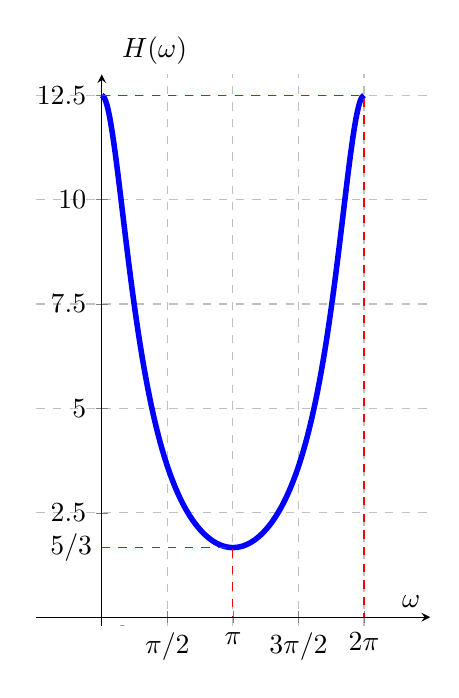
\begin{tikzpicture}
                    \begin{axis}[
                        axis lines = middle,
                        xlabel = {$\omega$},
                        ylabel = {$\abs{H(\omega)}$},
                        ylabel style={at={(rel axis cs:0.3, 1)}, anchor=south},
                        xmin = -0.2, xmax = 6.5,
                        ymin = -0.2, ymax = 13,
                        grid = major,
                        grid style = dashed,
                        scale only axis,
                        width = 5cm,
                        height = 7cm,
                        axis equal,
                        xtick = {0, 1.57, 3.14, 4.71, 6.28},
                        xticklabels = {$0$, $\pi/2$, $\pi$, $3\pi/2$, $2\pi$},
                        ytick = {0, 2.5, 5, 7.5, 10, 12.5},
                    ]
                    \addplot[domain=0:6.28, samples=100, smooth, line width=2pt, blue] {sqrt(17 + 8 * cos(deg(x))) / sqrt(1.5 + 0.2 * cos(deg(2 * x)) - 1.54 * cos(deg(x)))};
                    \addplot[dashed, red] coordinates {(0, 1.667) (3.14, 1.667) (3.14, 0)};
                    \addplot[dashed, red] coordinates {(0, 12.5) (6.28, 12.5) (6.28, 0)};
                    \node at (axis cs:0, 0) [anchor=north west] {O};
                    \node at (axis cs:0, 1.667) [anchor=east] {$5/3$};
                    \end{axis}
                \end{tikzpicture}
                \caption{作业 \thehomework~ 的系统幅频响应图}
                \label{fig:chap4-part2-homework3}
            \end{figure}
            由图可知,该系统是低通滤波器。
        \item 只有 ROC 为 $\abs{z} > 0.5$ 时,包含单位圆,该系统是稳定的;其余情况下系统是不稳定的。
    \end{enumerate}
\end{solution}

\begin{note}
    在本题中,如果使用 $H(z) = (1 + 4z^{-1})W(z)$,则解答过程如下:
    \begin{align*}
        W(z) = \frac{1}{1 - 0.7z^{-1} + 0.1z^{-2}} = \frac{5/3}{1 - 0.5z^{-1}} - \frac{2/3}{1 - 0.2z^{-1}},
    \end{align*}
    则
    \begin{align*}
        w(n) = \begin{cases}
            -\frac{5}{3}(0.5)^nu(-n - 1) + \frac{2}{3}(0.2)^nu(-n - 1), & \abs{z} < 0.2, \\
            -\frac{5}{3}(0.5)^nu(-n - 1) - \frac{2}{3}(0.2)^nu(n), & 0.2 < \abs{z} < 0.5, \\
            \frac{5}{3}(0.5)^nu(n) - \frac{2}{3}(0.2)^nu(n), & \abs{z} > 0.5.
        \end{cases}
    \end{align*}
    由于 $H(z) = (1 + 4z^{-1})W(z) = W(z) + 4z^{-1}W(z)$,故 $h(n) = w(n) + 4w(n - 1)$。
    因此,其单位冲激响应为
    \begin{align*}
        h(n) = \begin{cases}
            -\frac{5}{3}(0.5)^nu(-n - 1) + \frac{2}{3}(0.2)^nu(-n - 1) \\
            \quad - \frac{20}{3}(0.5)^{n - 1}u(-n) + \frac{8}{3}(0.2)^{n - 1}u(-n), & \abs{z} < 0.2, \\
            -\frac{5}{3}(0.5)^nu(-n - 1) - \frac{2}{3}(0.2)^nu(n) \\
            \quad - \frac{20}{3}(0.5)^{n - 1}u(-n) - \frac{8}{3}(0.2)^{n - 1}u(n - 1), & 0.2 < \abs{z} < 0.5, \\
            \frac{5}{3}(0.5)^nu(n) - \frac{2}{3}(0.2)^nu(n) \\
            \quad + \frac{20}{3}(0.5)^{n - 1}u(n - 1) - \frac{8}{3}(0.2)^{n - 1}u(n - 1), & \abs{z} > 0.5.
        \end{cases}
    \end{align*}
    其中只有 ROC 为 $0.2 < \abs{z} < 0.5$ 时,包含单位圆,该系统是稳定的;其余情况下系统是不稳定的。
\end{note}
